
In this chapter we will describe the different parts of the system and how the
identification algorithms will work.
%In this section we describe the user identification system. 
%This system provides a distributed and secure way to attain a user-password
%identification scheme like the ones commonly seen in centralized services.

\section{A Quasi-Identification Service}

% definition of a node and a service that is going to identify with it

Let A be a node of the DHT, and $S = \{S_1, S_2, \cdots, S_n\}$ a set of $n$
nodes that cooperate to provide a service. Let $NameofS$ be the name of service
$S$; every node that needs to use the service knows $NameofS$. $K_s =
SHA(NameofS)$ is the key that identifies $S$ in DHT, and $S_{root}$ is the node
closest to $K_s$ in the DHT. It follows that $S = \{S_1, S-2, \cdots, S_n\}$ is
composed of node $S_{root}$ and of all the nodes in its leafset. Let $I$ be a
identification service such that $I = \{ I_1, I_2, \cdots, I_n\}$ is a group of
$n$ nodes belonging to the DHT. 

% interaction between A, S & I, Figure and such

We suppose that the number of nodes that compose a service $S$ is fixed and does
not change over time. We also suppose that the same stands for any
quasi-identification service $I$.



% normal p2p networks provide storage for the peers inside but does not ensure
% control of capabilities, deletion nor modification of the files.

\section{Architectural principles}

\subsection{Securing the nodes of a leafset}

%% Refering to the section in the paper "A Scalable Architecture for Highly Reliable Certification"
The first step to requesting a service is to acquire the set of nodes that
compose the leafset for a giben root key $K$. Supposing that $K$ is associated
with node $K_{ROOT}$, there remains a probability for $K_{ROOT}$ to be
malicious. $K_{ROOT}$ might lie and provide references to other malicious nodes
in order to collude against the requester, or it might deny any service by
remaining silet. Therefore, a simple request to $K_{ROOT}$ will not suffice to
acquire a reliable leafset associated with $K$.

Our solution for mitigating this issue is to use the DiversityTrustedRoute
algorithm~\cite{diversity_trusted_route}. DiversityTrustedRoute uses different
nodes as starting points in order to reach the same root node $K_{ROOT}$. The
diversity of the routing tables on each node guarantees a very high probability
of reaching root node $K_{ROOT}$ using different paths, and therefore of
entering the leafset of $K_{ROOT}$ via different nodes. This makes for a more
secure way of acquiring the leafset associated with a key $K$.

\subsection{Normal service request}

Based on the services seen on~\cite{p2p_certification}, to find the nodes associated with a given
service, node $A$ computes the hash
of the service name: $K_s = SHA(ServiceName)$. Let $S_{root} $ be the node that
is closest to $K_s$ in the DHT. $A$ uses DiversityTrustedRoute to acquire the
leafset of $S_{root}$. $A$ thus obtains access to the set $S$ of nodes that
process requests for service $ServiceName$. Let L be the number of nodes in a
leafset: $card(S) = L + 1$.

Once $A$ has acquired $S$, it proceeds to the inception of its service request
by sending a $RequestInit$ message to every node in $S$. A $RequestInit$
message contains a public key $A^{pub}$ of client $A$. In reply to such a
message, every node $S_i$ sends its own public key $S^{pub}_i$. In order to
avoid man-in-the-middle attack, all the ensuing communications between $A$ and
nodes that belong to $S$ will use a public/private key encryption scheme to
ensure that no other node can read the content of the messages.
% later the node will use his user private key & public key in this exchange

If $A$ recieves at least $\frac{L}{2} + 1$ answers from the nodes in $S$, then
$A$ considers that the transaction will proceed. Since $S$ is composed of
common nodes from the DHT, it is possible for some of these nodes to be
malicious. However, as explained in our evaluation of the quasi identification
protocol~\ref{sec:evaluation}, a situation where $S$ contains more than
$\frac{L}{2}$ malicious nodes is highly improbable.

A combination of network failures and/or malicious nodes that choose to remain
silent may prevent $A$ from receiving at least $\frac{L}{2} + 1$ answers. Since
$S$ retains the properties of Pastry's leafset, the numerical closeness of its
nodes in the DHT implies that they will very likely be geographically far on
the Internet. Therefore, the probability of $\frac{L}{2} + 1 $ simultaneous IP
routing failures or node failures, that is the probability for more than
$\frac{L}{2}$ answers to not reach $A$, is very close to zero. To account for
this type of situation, $A$ aborts the transaction if it has not received a
sufficient amount of identical answers after a timeout $\delta t$. this is a
very rare and highly improbable case, as shown by our evaluation
in~\ref{sec:evaluation}.

%%%%%%% ---- OLD, NOT APPLICABLE TODAY ----
%%%The general view of the system consists in a multi-layered network based in trusted rings.
%%The general view of the system consists in a double-layered network; a Trusted
%%ring of nodes nested inside a normal DHT, with multiple routing policies
%%depending in the protocol of differents services. The user registration,
%%sign-in, logout and password change operations respectively allow a node to
%%register an user identity, to identify himself with an existing user identity,
%%to remove your user session and to change the password used to sign-in.
%%
%%The system needs to have a \textit{trusted ring} maintained by periodical
%%checks of capacity of his members to remain in the trusted ring and a
%%reputation system to evaluate this. Also, similar to the
%%leafset concept in Pastry, each trusted node needs to maintain a
%%\textit{trustset}, wich basically consist in D numerically closest trusted
%%nodes with D/2 clockwise nodes, and D/2 counter-clockwise ones.
%%
%%The system used to build the trusted node infraestructure in the P2P networks
%%needs to regularly asses the ability of the nodes to be part of the trusted
%%ring.
%%
%%The figure shows a basic structure of the system. There are normal nodes and
%%trusted nodes. Every trusted nodes maintains a \textit{trustsets}.


We now describe our protocols based on the system model. 
%Figure 2 shows the information objects and
%their storage locations, with arrows for the abstract flow of the
%login procedure, Table I lists the terms used in the algorithms.
%A. Account Registration

\section{Account registration}
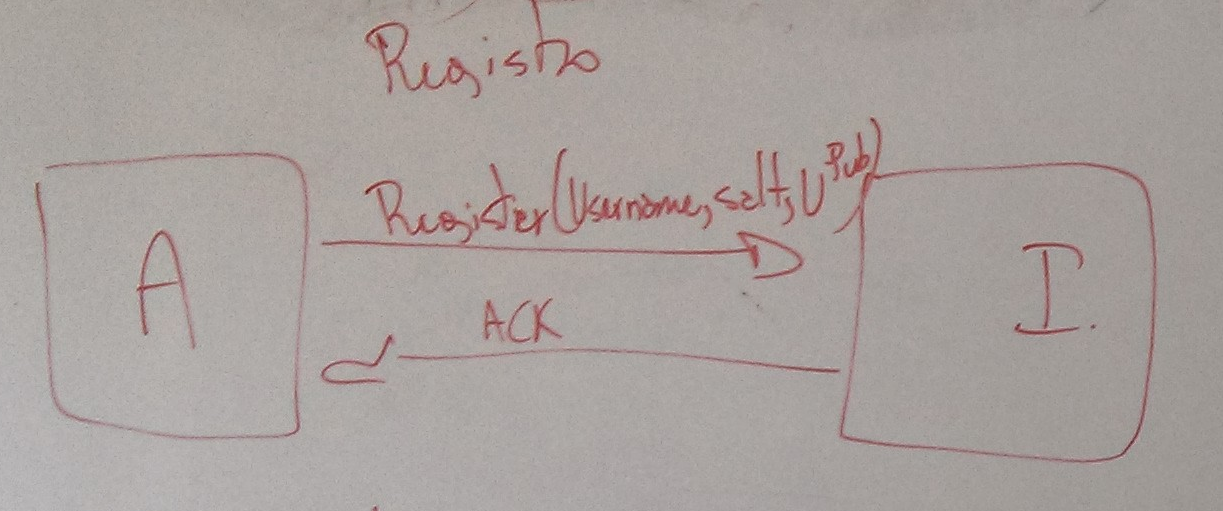
\includegraphics[width=14cm]{../img/registration_protocol_mockup.png}\\

To register a new user account ($U$), the node first
has to choose a \textit{username} and a \textit{password}.
%The \textit{username} should be unique in the network.
% The user checks if the username exists by sending a
% REGISTER(username, identity_file: [[c(user_keys_file), salt]).
% This operation use a accounted routing algorithm that uses only trusted
% nodes. When the register operation reaches the closest node to the username,
% it propagates a TRUSTSET_USERNAME_REGISTRATION operation. This operation sends a
% call to each node in the trustset of the node, wich then pass to do a council
% meeting. If the meeting results in favor, each of them sends a
% OK_USERNAME_REGISTRATION(user_identity_file_name) to node doing the REGISTER operation.
% 
% DETAILS OF THE REGISTER OPERATION
% DETAILS OF THE COUNCIL MEETING --> Explain before, in trusted node part 
% 

% key store file
Then, a key derivation process is issued to generate the user Private and
Public Keys. The
key derivation utilices a Salt ($U^{salt}$) and a Password ($U^{password}$) to
obtain the user's private and public Keys
($U^{priv}$ and $U^{pub}$).
The node  looks for the set $I$ set of nodes that will constitute the
identification service for the user $U$. To obtain the list of nodes that provides the user identification service for
the username $U^{username}$, the node $A$ computes its key $K$ such that $K =
SHA(U^{username})$. 

Then the node $A$ sends a request to every node $I_i$ in $I$ to register the
$U^{salt}$ and $U^{Pub}$ under the chosen  username  $U^{username}$. When the node
$A$ recieves at least $\frac{L}{2} + 1$ identical affirmative answers from
$I$ regarding the user registration, then $A$ assumes that the user was
actually registered.

%unique username
In case that the username was taken,
the node $A$ is prompted for a new username.


\section{Sign-in}

\subsection{User private key recovery}
\label{sec:private_key_recovery}
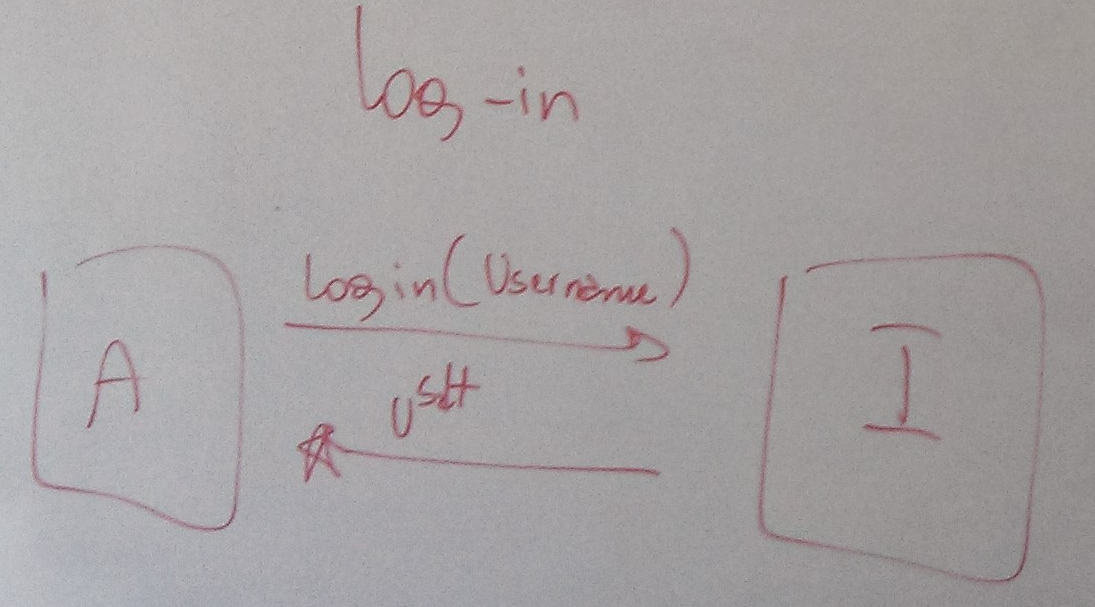
\includegraphics[width=14cm]{../img/login_protocol_mockup}\\

First, the node $A$ looks for the set $I$ set of nodes that will constitute the
identification service for the user $U$.
To obtain the list of nodes $I$ that provides the user identification service for
the username $U^{username}$, the node $A$ computes its key $K$ such that $K =
SHA(U^{username})$. 
Then the node $A$ sends a request to every node $I_i$ in $I$ to obtain the user
salt $U^{salt}$ needed to derive the user private key $U^{priv}$.
 When the node $A$ recieves at least $\frac{L}{2} + 1$ identical affirmative answers from
$I$ regarding the user salt, then $A$ assumes that the salt retrieved
corresponds to the one registered previously by the user ($U^{salt}$). Finally,
the node proccedes to derive the user private key $U^{priv}$ using his user password $U^{password}$.

\subsection{User identified service request}
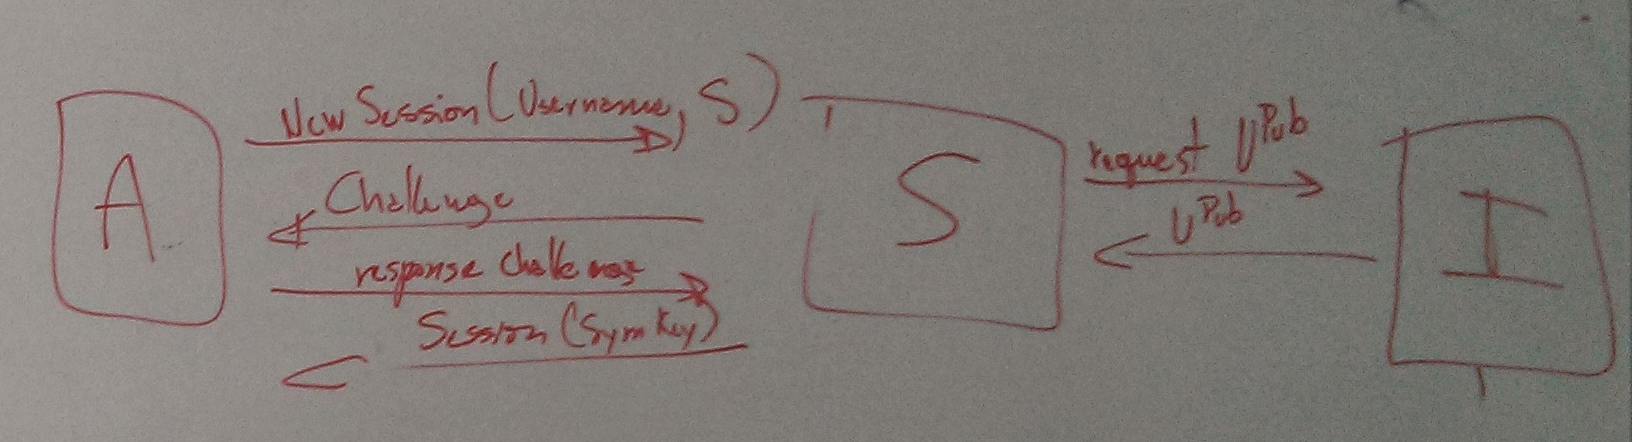
\includegraphics[width=14cm]{../img/session_creation_protocol_mockup}\\

Before carrying out a transaction for a client $A$, $S$ proceeds to
verify the identity of the client from another set $I$ of nodes. At the end of
the intentification process, the objective is to return a session key to $A$
and to store the created session on the nodes that belong $C$.

% CHALLENGE, TODO: FIND A BETTER ONE
Each node in $S$ generates a random secret $S^{secret}_i$ wich is sent to the
client $A$. Then, client $A$ responds each request with the corresponding secret
encrypted with his user private key $U^{priv}$, generating
$E^{secret_i}_{U^{priv}}$. 
%The service $S$ send a $EncryptedSecretRequest$ to the client $A$, wich is
%responded with the 
% The service requires a encrypted secret from the client A. The node A
encrypts the secret using his private key obtained through
\ref{sec:private_key_recovery}.

Upon reception of the $E^{secret_i}_{U^{priv}}$ message from the client $A$, every node in $S$
starts looking for the set $I$ of nodes that will constitute the quasi
identification authority. To determine wich nodes belong to $I$, $S$ computes
its key $K$ such that $K = SHA(U^{username})$. $I_{root}$ is the node closest
to $K$ in the DHT, and the quasi identification authority $I = \{ I_1, I_2,
\cdots, I_{L+1}\}$ for the identification of $A$ is composed of $I_{root}$
and its leafset secured through DiversityTrustedRoute.

Then each node in $S$ sends a request to every node $I_i$ in $I$ asking for the Username public key $U^{pub}$. When a node
$S_i$ of $S$ recieves at least $\frac{L}{2} + 1$ identical answers from
$I$ regarding the $U^{pub}$, then $S_i$ assumes that the public key recieved
actually corresponds to the Username being identified. Each node $S_i$ in $S$
uses the $U^{pub}$ to decrypt $E^{secret_i}_{U^{priv}}$. If the result matches
the shared random secret $S^{secret}_i$, $S_i$ recognizes the node $A$ as the
user $U$.


\section{Logout}
The session are maintained by each service the user identified with. To close a
session, the node identified as the user $U$ sends a session close request to
the service $S$ using the session keys for the transaction. Also, the sessions
keys are issued for a certain time. After that time is passed, the node needs
to ask for a new session key with the service.

%%%%%%%%%%%%%   Peerson Passwords in P2P networks %%%%%%%%%%%%%
%% A problem related to logging out is revoking remembered
%%credentials on another device, e. g., a user’s stolen phone. To
%%accomplish this, we first run the password change operation,
%%which locks out all devices with remembered logins, because
%%he key store key KKS changed (as well as the filename fKS ).
%%Next, we use the device mapping devmap to inform all devices
%%about the new key (and filename), except the device that is to
%%be revoked. To inform a device about the change, we update
%%the corresponding values in the device’s login information file
%% FDL which can be accessed from the device by using the
%%locally stored credentials.
%% Algorithm 4 describes this necessary extension. After run- the password change
%%operation, all devices that not ning shouldbe revoked and that have remembered
%%logins (and therefore are devmap) referenced in the device mapping are
%%processed. The device login information filename fDL and its key KDL are read,
%%and the new key store key KKS new and filename fKS new are written to the
%%device login information file FDL, encrypted under the device key KDL.
%%Finally, the modified devmap is saved back to the login information file FLI.
%%%%%%%%%%%%%   Peerson Passwords in P2P networks %%%%%%%%%%%%%
 

\section{Password Change}

First, the node $A$ needs to recover his actual private key using the proccess
in~\ref{sec:private_key_recovery}. Then the node $A$ generates a new private/public
key pair using the new password.  With this, the node $A$ request a
password change to every node $I_i$ in $I$. The request is signed with the
actual user private keys, and includes the new user public key $U^{pub}_{new}$
and salt used to derive his new private key $U^{salt}_{new}$. 
 When the node $A$ recieves at least $\frac{L}{2} + 1$ identical affirmative
answers from $I$ regarding the user password change, then $A$ assumes that the
user keys (and password) were updated.


%%%%%%%%%%%%%   Peerson Passwords in P2P networks %%%%%%%%%%%%%
%%Before the user can change the password, she must log in using her password to
%%obtain KLI . With this information, the password change can be accomplished
%%(see Algorithm 3): the user is asked for a new password and a new salt is
%%generated. The key-derivation function is used to generate a new key KLI new
%%for the login information file. Then, the content of the key-store file is
%%fetched and decrypted (with the old key). A new key KKS new is generated and
%%used for encrypting the key-store content again before it is saved to the
%%storage system, obtaining a new filename fKS new.
%%Finally, the login information file
%%is updated: fKS new, KKS new, the write credential KW as well as a new empty
%%device mapping devmapnew are encrypted with the new key KLI new.
%%  Together with the new salt, this ciphertext is written to the distributed
%%storage, using the reference fLI and the credential KW, to authenticate the
%%write operation. Lastly, the keys stored in the key store should be updated by
%%the application using our P2P protocol.  See Section VI-E for a discussion. At
%%this point, old device login information files can also be deleted from the
%%storage to reclaim space.
%%%%%%%%%%%%%   Peerson Passwords in P2P networks %%%%%%%%%%%%%

\section{Lazy User's Information Store Maintenance}
Insertions and departures of nodes in the DHT cause modifications of the
leafsets, and it is therefore crucial to maintain the consistency of the user's
information $S_{username}$ used for his identification procedures. The user's information
consists in the user's public keys and salt. This has to be done on every node in the identification service
$I$.\\

Upon entering a leafset, a node $X$ must update its own view of the user's
information. Analog to the lazy log consistency maintenance procedure seen
in~\cite{p2p_certification}, it starts by following the steps below to find
which user's information store must be updated.\\

\textit{Step 1:} $X$ constructs the set of nodes
$N = \{ X_{-L/2}, X_{-L/2 +1}, \cdots, X, \cdots X_{L/2 -1}, X_{L/2} $
composed of its leafset, and of the $\frac{L}{2} +1$ nodes both on the right
side and on the left of its leafset. 
%% TODO: figure example  of this
In order to build this set of nodes, $X$ can ask the farthest nodes $X_{-L/2}$
and $X_{L/2}$ of its leafset for their own respective leafsets. If one of these
nodes fails to answer in a timely manner, $X$ can ask the second to farthest
node, and so on until its immediate neighbors in the leafset. Having
$\frac{L}{2} +1$ malicious neighbors on both sides is highly improbable, and
practically infeasible: for more details about this statement, please refer to
our probabilistic evaluation in section~\eqref{sec:eval_lazy_maintenance}. \\

\textit{Step 2:} $X$ computes interval $L$ such that
$$
L = [ X_{-L/2} - \frac{| X_{-L/2} - X_{-L/2 +1} |}{2}, X_{L/2} +\frac{|
X_{L/2} - X_{L/2 -1} |}{2} ]
$$


and sends it to every node in set $N$. Upon reception of this message, every
node replies with a set of all the usernames $U^{username} \in L$ it
stores, along with the last information regarding the user's
information corresponding to each username. Thus the format of a response is a
variable-size set of pairs $\{ U^{username}, S_{username}\}$.\\


\textit{Step 3:} $X$ builds set 
$Y =  \{ \{U^{username_i}, S_{username_i}\},\cdots,\{ U^{username_j},
S_{username_j}\} \} $ the union of all recieved usernames and user's
information. $X$ then discards all pairs $\{ U^{username}, S_{username}\}$ that
appear less than $\frac{L}{2} +1$ times in $Y$, since these may have been
generated by colluding nodes. Once this is done, $X$ synchronizes all the
user's information store whose username matches one of the remaining usernames
in set $Y$.

% checkpoints
For every user information that $X$ must synchronize, $X$ selects a node $Z$ in $N$ that
holds this user information. If $X$ does not have any entry for this username,
then $X$ must ask $Z$ for the entire user's information store. Otherwise, $X$
sends the last $q$ public keys and salts it has of the user.

%% TODO: complete this
